% !TEX root = DesignDocument.tex

\chapter{User Documentation}

\section{Overall Guide}
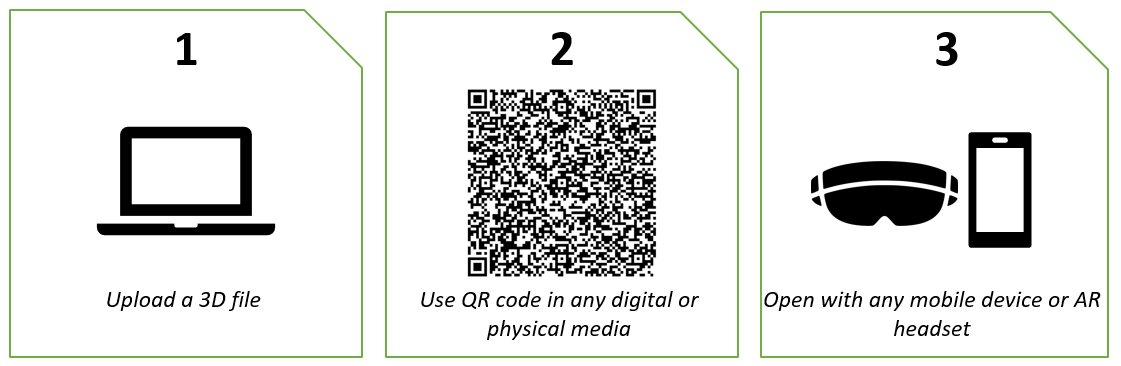
\includegraphics[width=\textwidth]{AugmentedEducationHowTo.png}

\section{User Guide for Website}
\begin{itemize}
    \item Public Content: displays all publicly viewable files.
    \begin{itemize}
        \item Displayed files may be searched or filtered using the Search and Filter bar at the top of the listing.
        \item Clicking a file will reveal options for selecting a file type in which to downloaded the file or for which to a have a linked QR code generated.
        \item QR codes must be generated for mobile devices and all non-mobile devices separately. 
    \end{itemize}
    \item My Content: displays a user's public and private files.
    \begin{itemize}
        \item User's private and public files are displayed in separate tables.  
        \item Tables may be searched or filtered using the Search and Filter bar at the top of the listings.
        \item Clicking a file will reveal options for selecting a file type in which to downloaded the file or for which to a have a linked QR code generated.
        \item QR codes must be generated for mobile devices and all non-mobile devices separately. 
        \item Clicking a file will reveal an options for deleting a file from the cloud. Any QR codes previously associated with the file will no longer work. 
    \end{itemize}
    \item Upload: allows a user to upload a file.
    \begin{enumerate}
        \item Add a file to be uploaded.  
        \item Optionally add a material file to be uploaded. 
        \item Optionally add an alternate display name for the file.
        \item Optionally add a description for the file.
        \item Select whether the file will be public or private.
        \item Press "Upload."
        \item A notification message will appear to indicate success or failure of the upload. 
    \end{enumerate}
    \item Help: displays platform guide for users. 
\end{itemize}

\section{User Guide for HoloLens}

\section{User Guide for Mobile App}
There are four main screens available in the mobile app. These are the login, file listing, QR code reader, and AR view. 
\begin{itemize}
    \item Login Screen
    \begin{itemize}
        \item You may log in using credentials for an account created on the website. Credentials will be saved after the app is closed if you check the box.
        \item Alternatively, you may "Continue Offline" if you don't have a login or don't need to sign in. 
        \item Offline users can view files that are already downloaded on the device and scan new QR codes for adding more models to their list.
    \end{itemize}
    \item File Listing
    \begin{itemize}
        \item The files available to view are listed here.
        \item Some files are already downloaded on the device, and some files are available from the website.
        \item In offline mode, only downloaded files will appear.
        \item A user can select a file from the list. A file that is already downloaded will load in the AR View screen. A file that is not downloaded will be downloaded while a loading spinner appears to demonstrate that the download is in progress.
        \item There is a button available to access the QR Code Reader screen.
    \end{itemize}
    \item QR Code Reader
    \begin{itemize}
        \item The whole screen will be a live feed from the camera.
        \item The user can point their device at a mobile QR code and the app will automatically scan it, returning the user to the File Listing with the new file added.
        \item A user may use the back navigation button to return to the file listing if they choose not to scan a QR code.
    \end{itemize}
    \item AR View
    \begin{itemize}
        \item The AR view allows the user to view the 3D model in their own environment.
        \item The view will have a live feed from the phone's camera.
        \item Small blue points will appear as the phone maps out surfaces.
        \item The user may need to move the device around slowly and allow the phone a few seconds to map flat horizontal surfaces.
        \item When the trigrid appears over the surfaces, the user can tap the screen where they would like to place the model.
        \item After the model is placed, they can use the + and - buttons to change the size, as well as use the number input at the bottom to change how quickly the scale changes.
        \item The user should be able to move around the placed object to see it from different sides, while it remains anchored where it was placed.
        \item If the user covers the camera or turns too far away, the model may lose tracking and need to be replaced.
        \item The user may use the back navigation button to return to the file listing.
    \end{itemize}
\end{itemize}

\section{Demos}

See Appendix \ref{ch:support} for demonstrations of the platform in use. 

\section{User Guide for Capturing Demos}

\subsection{Website}
\begin{itemize}
    \item For screenshots:
    \begin{enumerate}
        \item Navigate to the desired page. 
        \item Find and open Snipping Tool, a default application on windows. 
        \item Select "New" and then select the capture area. 
        \item Save or right-click to copy screenshot. 
    \end{enumerate}
    \item For videos:
    \begin{enumerate}
        \item Open Microsoft PowerPoint.
        \item Navigate to the "Insert" tab. 
        \item Select "Screen Recording." 
        \item Select the recording area.
        \item Press "Record."
        \item To end recording, press the Window's logo key, shift, and "Q" all together.
        \item The recording will now appear in your PowerPoint. 
        \item To save the recording to your desktop, right-click it and select "Save media as..."
    \end{enumerate}
\end{itemize}

\subsection{HoloLens}
\begin{enumerate}
    \item With the HoloLens on, verbally say "Cortana, record this," to begin recording.
    \item Perform the "bloom" motion of opening a closed fist to finish recording.
	\item Recordings will be saved to the One Drive of the account signed in on the HoloLens. Access the One Drive to share and view recordings. 
\end{enumerate}

\subsection{Mobile App}
\begin{enumerate}
    \item Download any screen recording application. 
    \item Open the screen recording application and press the "record" icon.
    \item To finish recording, press the "record" icon again. 
    \item Select "Save."
    \item The video will be saved to the mobile device's gallery and may be shared.
\end{enumerate}